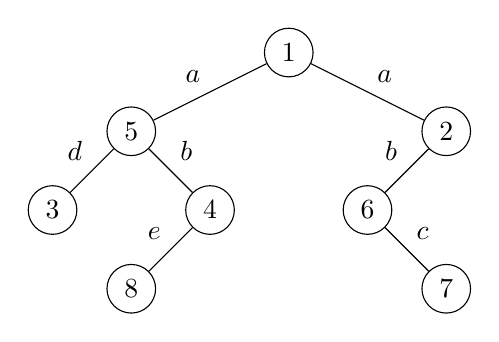
\begin{tikzpicture}

\node[circle, draw=black] (1) at (5, 5) {1};
\node[circle, draw=black] (5) at (3, 4) {5};
\node[circle, draw=black] (2) at (7, 4) {2};
\node[circle, draw=black] (3) at (2, 3) {3};
\node[circle, draw=black] (4) at (4, 3) {4};
\node[circle, draw=black] (6) at (6, 3) {6};
\node[circle, draw=black] (8) at (3, 2) {8};
\node[circle, draw=black] (7) at (7, 2) {7};

\draw (1) -- (2) node[midway, above right] {$a$};
\draw (2) -- (6) node[midway, above left] {$b$};
\draw (6) -- (7) node[midway, above right] {$c$};
\draw (1) -- (5) node[midway, above left] {$a$};
\draw (5) -- (4) node[midway, above right] {$b$};
\draw (4) -- (8) node[midway, above left] {$e$};
\draw (5) -- (3) node[midway, above left] {$d$};
%1-a-2-b-6-c-7
%|
%a
%|
%5-b-4-e-8
%|
%d
%|
%3

\end{tikzpicture}